\chapter{Application des méthodes au problème}
    Dans cette partie, nous allons présenter comment les diverses techniques que nous souhaitons appliquer sont compatibles avec notre cas spécifique du sudoku.
    \section{A*}
    Comme vu précédemment, l'algorithme A* est un algorithme de recherche de plus court chemin dans un graphe. Plus précisément dans le cas du Sudoku, on construit un graphe ayant pour racine la \textbf{grille initiale}, avec seulement les indications de départ.\\
            Chaque sommet correspond ensuite à un état de la grille, parmi lesquels on avance en ajoutant un chiffre dans une case vide. On va donc de case en case jusqu'à ce que la grille soit complète ou que l'on ai trouvé une erreur, au quel cas on retourne en arrière et on retente une autre possibilité.
            \bigskip
            Sans revenir sur l'algorithme lui même, il est tout de même nécessaire de préciser certains points : $A^*$ utilise \textbf{deux listes}, une dites \textit{fermée} et l'autre \textit{ouverte}. \textit{La liste ouverte contient toutes les grilles de sudoku qui ont été évaluées mais pas développées. La liste fermée contient quand à elle l'ensemble des grilles qui ont été étudiées.}\\
            Pour déterminer quel chemin emprunter l'algorithme calcul un \textbf{coût} $F$ pour chaque sommet et on cherche en cherche le minimum à chaque étape. \textit{Remarque : on calcule le coût de chaque successeur c'est à dire en remplissant une case vide avec un chiffre entre 1 et 9 afin de déterminer laquelle est ``optimale'' pour continuer la recherche.} Le coût $F$ est déterminé comme la somme d'une fonction coût $G$ et d'une heuristique $H$.
            \bigskip
            La seule particularité de cette application de $A^*$ est que l'on doit, pour chaque case optimale choisie, tester toutes les possibilités de valeurs de possibles. Tant que l'on a pas trouvé de solution ou que l'on ai testé toute les grilles possibles, l'algorithme va :
            \begin{itemize}
                \item actualiser les listes ouverte et fermée ainsi que les valeurs possibles des cases vides,
                \item trouver la grille ayant la plus petite valeur pour $F$,
                \item créer des grilles à partir de la grille précédente \textit{(on assigne aussi celle-ci comme parent de la nouvelle grille)} et d'une des valeurs possibles pour la case ``optimale'',
                \item vérifier la présence de doublon, si c'est le cas, il faut renvoyer une erreur, tester les autres possibilités et éventuellement remonter au niveau du parent pour essayer ses autres possibilités.
                \item s'il n'y a pas de doublon, on recommence la recherche de case ``optimale'' dans la nouvelle grille \textit{(via récursivité)}
            \end{itemize}
        \subsection{Choix des fonctions coût}
            On peut choisir différentes fonction coût pour le problème du Sudoku, ce choix va bien sur affecté le temps de calcul de l'algorithme.
            \subsubsection*{La fonction G}
                L'une des façons la plus simple de l'estimer est de prendre le nombre de cases remplies dans la grille. En effet, moins il y a de case vide, plus il sera simple de déterminer une valeur.
            \subsubsection*{L'heuristique H}
                C'est principalement le choix de l'heuristique qui influe sur l'efficacité de l'algorithme, notre premier choix est une fonction qui renvoie le nombre de valeurs possibles pour chacune des cases de la grille testée \textit{(valeurs comprises entre $1$ et $9$)}. On va choisir de remplir la case ayant le moins de possibilité comme étant la grille suivante à développer.\\
                Cette valeur est déterminée selon les règles du Sudoku \textit{(une seule apparition par ligne, colonne ou bloc)} et les cases contenues dans la liste fermée \textit{(les cases remplies de la grille)}.\\
                \textit{Remarque : dans le cas où il n'y a aucune possibilité, c'est que l'on a trouvé une erreur, on renverra alors la valeur $9$ ainsi qu'un message d'erreur.}
        \subsection{Implémentation}
            \subsubsection{Diagramme de classe}
                \begin{center}
                    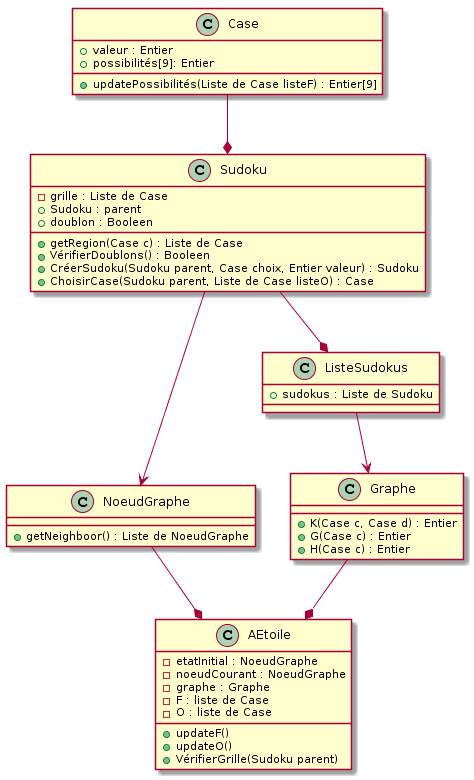
\includegraphics[scale = 0.5]{images/AstarDiagrammeClasse.png}
                \end{center}
                \bigskip
                \begin{description}
                    \item[Case]: C'est un emplacement pouvant recevoir une \textit{valeur} comprise entre $1$ et $9$. Chaque Case possède un tableau de $9$ entiers \textit{possibilités[]}, initialisé à $\{1,2,3,4,5,6,7,8,9\}$.\\
                        La fonction \textit{updatePossibilités()} met à jour les valeurs possibles de la Case, en fonction des Cases contenues dans la liste fermée. Si une valeur est impossible, on la remplace par $0$ dans \textit{possibilités[]}.
                    \item[Sudoku]: Il s'agit tout d'abord d'une \textit{grille}, une liste de 81 Cases, ainsi qu'un booléen \textit{doublon}. On utilise aussi une référence au Sudoku \textit{parent}, celui qui à permit d'obtenir ce Sudoku.\\
                        La fonction \textit{getRégion(Case c)} renvoie la liste des autres Cases contenues dans la même région que la Case c \textit{(dans la ligne, la colonne et le bloc)}.\\
                        Comme son nom l'indique, \textit{VérifierDoublon()} va tester la présence de doublon dans une ligne, une colonne ou un bloc de la grille.\\
                        \textit{CréerSudoku(Sudoku parent, Case choix, Entier valeur)} construit un nouveau Sudoku à partir du Sudoku \textit{parent}, en lui ajoutant le chiffre \textit{valeur} dans la Case vide \textit{choix}.\\
                        Enfin, \textit{ChoisirCase(Sudoku parent, Liste de Case listeO)} détermine quelle Case de \textit{listeO} est ``optimale'' pour le prochain déplacement depuis \textit{parent}, c'est ici que l'on va chercher le minimum de $F=G+H$.\\
                    \textit{La classe Sudoku hérite de la classe NoeudGraphe, contenant un fonction qui renvoie les NoeudGraphes voisins d'un NoeudGraphe.}
                        \item[ListeSudokus]: On maintient simplement une liste de tout les Sudokus construis.\\
                    \textit{ListeSudokus hérite de la classe Graphe, qui contient les méthodes permettant de calculer $G$ et $H$}
                    \item[AEtoile]: Possède un \textit{etatInitial}, le NoeudGraphe qui correspond à la grille de départ, un Graphe et un NoeudGraphe \textit{noeudCourant}. C'est dans cette classe que sont définit les listes de Cases \textit{listeFermée} et \textit{listeeOuverte}, ainsi que les méthodes pour les mettre à jour.\\
                        La fonction \textit{VérifierGrille(Sudoku parent)} est la fonction récursive principale de l'algorithme, celle qui va appeler \textit{ChoisirCase()}, \textit{CréerSudoku()} et \textit{VérifierDoublon()}.
                \end{description}
            \subsubsection{Diagramme de séquences}
                \begin{center}
                    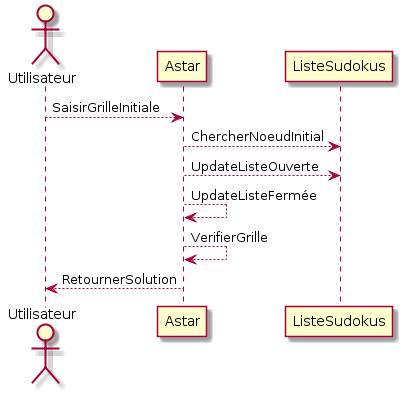
\includegraphics[scale=0.5]{images/AstarDiagrammeSequences.png}
                \end{center}
                Dans ce diagramme de séquence nous voyons bien que l'utilisateur commence par saisir sa grille. Nous avons donc le noeud initial de notre algorithme. Ensuite 
    \section{Algorithme génétique}
        Pour spécifier notre instance générale d'algorithme génétique, nous avons 4 éléments à définir:
        \begin{itemize}
            \item Les génomes
            \item La sélection des meilleurs génomes
            \item Le croisement de différents génomes
            \item La mutation d'un génome
        \end{itemize}
        Pour certains de ces éléments, il peut exister différentes manières de procéder, nous allons donc en détailler plusieurs.
        \subsection{Génomes}
            Dans un premier temps, il nous faut nous poser la question de comment représenter notre grille de sudoku sous un format propice à un algorithme génétique.\\
            \subsubsection{Méthode 1D}
                Dans beaucoup de cas, travailler sur un tableau à une dimension simplifie énormément le travail. Nous allons donc procéder comme suit:
                \begin{description}
                    \item[Grille sudoku vide]:\\
                        \begin{center}
                            \begin{tabular}{|c|c|c| |c|c|c| |c|c|c|}
                                \hline
                                &\textbf{1}&&&&\textbf{3}&&&\\
                                \hline
                                &&&\textbf{4}&&&&&\\
                                \hline
                                &&&&\textbf{2}&&&&\\
                                \hline
                                \hline
                                &&&\textbf{7}&&&&&\\
                                \hline
                                \textbf{8}&&&&&&&\textbf{6}&\\
                                \hline
                                &&\textbf{5}&&&&&&\\
                                \hline
                                \hline
                                &&&&\textbf{3}&&&&\textbf{9}\\
                                \hline
                                &\textbf{3}&&&&&\textbf{1}&&\\
                                \hline
                                &&&&\textbf{6}&&&&\\
                                \hline
                            \end    {tabular}
                        \end{center}
                    \item[G\'enome]: Un tableau d'une dimension contenant uniquement le contenu des cases \textbf{non données} dans l'énonce.
                \end{description}
            \subsubsection{Méthode 2D}
                Cependant il subsiste des cas où il est important de garder l'aspect 2D pour faciliter les traitements qui seront fait dessus par la suite.\\
                Dans ces cas ci, on garde un tableau 2D de ``cases'', qui seront une pair contenant une valeur, et si cette case est donnée dans l'énoncé
        \subsection{Sélection}
            La sélection est une étape qui ne devrait pas être trop complexe.\\
            Le but serait d'affecter à chaque grille un \textbf{score}, tel que le score ``parfait'' corresponde à la une grille complétée, et plus la grille serait ``résolue'', plus le score serait élevé, plus la grille serait proche de la résolution.\\

            Une fois ce score obtenu, il nous suffira de prendre la \textbf{meilleure moitié} de la génération actuelle (Ceux dont le score est le plus élevé).\\

            Sachant que une grille résolue est une grille ``Avec 9 chiffres différents par ligne, colonne, et bloc''.\\
            Nous allons donc définir le score comme étant la somme du nombre de chiffres différents par lignes, colonnes, et blocs.

            \begin{center}
                \begin{tabular}{rcl}
                    \textbf{Score}&=&$\sum_{i=1}^9$\textbf{nombre numéros différents dans ligne i}\\
                        &+&$\sum_{i=1}^9$\textbf{nombre numéros différents dans colonne i}\\
                        &+&$\sum_{i=1}^9$\textbf{nombre numéros différents dans bloc i}
                \end{tabular}
            \end{center}
        \subsection{Croisement}
            Le croisement des génomes sélectionnés est la méthode la plus importante de tout l'algorithme, car c'est la méthodes qui sera en charge de ``passer'' les gains d'information précédents aux nouveaux génomes.\\
            Il parait normal que le croisement ne soit pas réalisé tout le temps, c'est la raison pour laquelle nous allons imposer un \textbf{taux de croisement}.\\
            Ce taux ($0\leq taux\leq 1$) est défini par l'utilisateur, et représente le pourcentage de chance qu'une paire de génomes se croise.\\

            Nous commençons par diviser d'intégralité des génomes sélectionnés en \textbf{paires distinctes de génomes}.\\
            Cela nous évitera que le même génome se retrouve plusieurs fois au sein de croisement.\\

            Deux méthodes peuvent être employées pour le croisement:
            \begin{itemize}
                \item Croisement naïf
                \item Croisement optimisé
            \end{itemize}
            \subsubsection{Croisement naïf}
                Ce croisement utilise un génome basé sur le modèle 1D.\\
                Le but de ce dernier est de fonctionner rapidement, et à défaut d'être efficace rapidement, il utilise l'aléatoire pour favoriser un mélange hétéroclite sur plusieurs générations.\\
                \subsubsubsection{Fonctionnement}
                    Donnons nous 2 génomes tirés aléatoirement parmi ceux sélectionnés lors de la phase précédente.\\
                    \begin{description}
                        \item[Genome 1]:\\
                            \[
                                \begin{array}{|c|c|c|c|c|c|c|c|c|c|}
                                    \hline
                                    g_1&g_2&g_3&g_4&g_5&g_5&g_6&\cdots&g_{n-1}&g_{n}\\
                                    \hline
                                \end{array}
                            \]
                        \item[Genome 2]:\\
                            \[
                                \begin{array}{|c|c|c|c|c|c|c|c|c|c|}
                                    \hline
                                    h_1&h_2&h_3&h_4&h_5&h_5&h_6&\cdots&h_{n-1}&h_{n}\\
                                    \hline
                                \end{array}
                            \]
                    \end{description}

                    L'algorithme sélectionne alors un nombre k tel que: $1\leq k\leq n$.\\
                    Ce nombre servira de point de séparation pour les deux génomes.
                    \begin{description}
                        \item[Genome 1]:\\
                            \[
                                \begin{array}{|c|c|c|c|c|c|c|c|c|c|}
                                    \hline
                                    g_1&g_2&g_3&\cdots&g_{k-1}&g_k&g_{k+1}&\cdots&g_{n-1}&g_{n}\\
                                    \hline
                                \end{array}
                            \]
                        \item[Genome 2]:\\
                            \[
                                \begin{array}{|c|c|c|c|c|c|c|c|c|c|}
                                    \hline
                                    h_1&h_2&h_3&\cdots&h_{k-1}&h_k&h_{k+1}&\cdots&h_{n-1}&h_{n}\\
                                    \hline
                                \end{array}
                            \]
                    \end{description}

                    En croisant les deux moitiés, nous pouvons donc créer deux nouveau génomes reprenant les gènes des parents.
                    \begin{description}
                        \item[Nouveau genome 1]:\\
                            \[
                                \begin{array}{|c|c|c|c|c|c|c|c|c|c|}
                                    \hline
                                    g_1&g_2&g_3&\cdots&g_{k-1}&g_k&h_{k+1}&\cdots&h_{n-1}&h_{n}\\
                                    \hline
                                \end{array}
                            \]
                        \item[Nouveau genome 2]:\\
                            \[
                                \begin{array}{|c|c|c|c|c|c|c|c|c|c|}
                                    \hline
                                    h_1&h_2&h_3&\cdots&h_{k-1}&h_k&g_{k+1}&\cdots&g_{n-1}&g_{n}\\
                                    \hline
                                \end{array}
                            \]
                    \end{description}
                \subsubsubsection{Inconvénients}
                    Malheureusement, aussi simple soit elle, elle est loin d'être la meilleure.\\
                    En effet, elle prend de manière anarchique et aléatoire les gènes des parents. Comment être sûr de ce que nous avons pris?\\
                    Ce qui faisait le ``haut score'' des parents se retrouvera peut être détruit par ce croisement (Modification d'une ligne, colonne ou bloc qui était résolu)
            \subsubsection{Croisement optimisé}
                Pour palier à cette perte d'information, nous allons mettre en place une autre méthodologie.\\
                Et si au lieu de croiser naïvement, nous faisions attention à préserver des parties intéressantes?
                \subsubsubsection{Pré-requis}
                    Nous allons donc faire un croisement qui part d'une supposition simple:\\
                    \begin{center}
                        Tous les génomes sont valides pour les blocs
                    \end{center}
                    Générer une première génération respectant cette condition est relativement facile (Pour chaque bloc, regarder les nombres pas encore placés, et les mettre 1 par case vide).\\
                    Il faudra juste faire attention à préserver cette propriété lors du croisement.
                    Le croisement se fera sur un modèle 2D, pour garder cette idée de correct du point de vue des blocs.\\
                \subsubsubsection{Mise en place}
                    Le croisement sélectionnera au hasard 2 génomes parmi les parents, et en calculera un ``score'' de ligne et colonne:\\
                    \begin{description}
                        \item[Parent 1]:\\
                            \begin{center}
                                \begin{tabular}{|c|c|c| |c|c|c| |c|c|c| |l}
                                    \hline
                                    X&\textbf{G}&X&X&X&\textbf{G}&X&X&X&$\rightarrow l_1$\\
                                    \hline
                                    X&X&X&\textbf{G}&X&X&X&X&X&$\rightarrow l_2$\\
                                    \hline
                                    X&X&X&X&\textbf{G}&X&X&X&X&$\rightarrow l_3$\\
                                    \hline
                                    \hline
                                    X&X&X&\textbf{G}&X&X&X&X&X&$\rightarrow l_4$\\
                                    \hline
                                    \textbf{G}&X&X&X&X&X&X&\textbf{G}&X&$\rightarrow l_5$\\
                                    \hline
                                    X&X&\textbf{G}&X&X&X&X&X&X&$\rightarrow l_6$\\
                                    \hline
                                    \hline
                                    X&X&X&X&\textbf{G}&X&X&X&\textbf{G}&$\rightarrow l_7$\\
                                    \hline
                                    X&\textbf{G}&X&X&X&X&\textbf{G}&X&X&$\rightarrow l_8$\\
                                    \hline
                                    X&X&X&X&\textbf{G}&X&X&X&X&$\rightarrow l_9$\\
                                    \hline
                                    \hline
                                    $\downarrow$&$\downarrow$&$\downarrow$&$\downarrow$&$\downarrow$&$\downarrow$&$\downarrow$&$\downarrow$&$\downarrow$&\\
                                    $c_1$&$c_2$&$c_3$&$c_4$&$c_5$&$c_6$&$c_7$&$c_8$&$c_9$&\\
                                \end{tabular}
                            \end{center}
                        \item[Parent 2]:\\
                            \begin{center}
                                \begin{tabular}{|c|c|c| |c|c|c| |c|c|c| |l}
                                    \hline
                                    Y&\textbf{G}&Y&Y&Y&\textbf{G}&Y&Y&Y&$\rightarrow l_1$\\
                                    \hline
                                    Y&Y&Y&\textbf{G}&Y&Y&Y&Y&Y&$\rightarrow l_2$\\
                                    \hline
                                    Y&Y&Y&Y&\textbf{G}&Y&Y&Y&Y&$\rightarrow l_3$\\
                                    \hline
                                    \hline
                                    Y&Y&Y&\textbf{G}&Y&Y&Y&Y&Y&$\rightarrow l_4$\\
                                    \hline
                                    \textbf{G}&Y&Y&Y&Y&Y&Y&\textbf{G}&Y&$\rightarrow l_5$\\
                                    \hline
                                    Y&Y&\textbf{G}&Y&Y&Y&Y&Y&Y&$\rightarrow l_6$\\
                                    \hline
                                    \hline
                                    Y&Y&Y&Y&\textbf{G}&Y&Y&Y&\textbf{G}&$\rightarrow l_7$\\
                                    \hline
                                    Y&\textbf{G}&Y&Y&Y&Y&\textbf{G}&Y&Y&$\rightarrow l_8$\\
                                    \hline
                                    Y&Y&Y&Y&\textbf{G}&Y&Y&Y&Y&$\rightarrow l_9$\\
                                    \hline
                                    \hline
                                    $\downarrow$&$\downarrow$&$\downarrow$&$\downarrow$&$\downarrow$&$\downarrow$&$\downarrow$&$\downarrow$&$\downarrow$&\\
                                    $c_1$&$c_2$&$c_3$&$c_4$&$c_5$&$c_6$&$c_7$&$c_8$&$c_9$&\\
                                \end{tabular}
                            \end{center}
                    \end{description}
                    Où ``\textbf{G}'' représente un chiffre donné dans l'énoncé, et ou $l_x$ et $c_x$ représentent les scores de la ligne/colonne $x$.\\
                    $l_x$ et $c_x$ seront calculés comme le nombre d'éléments différents par ligne et colonne. Cela signifie donc que $1\leq l_x, c_x\leq 9$\\

                    Nous allons alors réunir les lignes et colonnes en lignes et colonnes de blocs.
                    \begin{description}
                        \item[Parent 1]:\\
                            \begin{center}
                                \begin{tabular}{|c|c|c| |l}
                                    \hline
                                    X&X&X&$\rightarrow L_1$\\
                                    \hline
                                    X&X&X&$\rightarrow L_2$\\
                                    \hline
                                    X&X&X&$\rightarrow L_3$\\
                                    \hline
                                    \hline
                                    $\downarrow$&$\downarrow$&$\downarrow$&\\
                                    $C_1$&$C_2$&$C_3$&\\
                                \end{tabular}
                            \end{center}
                        \item[Parent 2]:\\
                            \begin{center}
                                \begin{tabular}{|c|c|c| |l}
                                    \hline
                                    Y&Y&Y&$\rightarrow L_1$\\
                                    \hline
                                    Y&Y&Y&$\rightarrow L_2$\\
                                    \hline
                                    Y&Y&Y&$\rightarrow L_3$\\
                                    \hline
                                    \hline
                                    $\downarrow$&$\downarrow$&$\downarrow$&\\
                                    $C_1$&$C_2$&$C_3$&\\
                                \end{tabular}
                            \end{center}
                    \end{description}
                    Où $L_x=\sum_{i=x}^{i=x+2}l_i$ et $C_x=\sum_{i=x}^{i=x+2}c_i$.
                \subsubsubsection{Génération des fils}
                    En prenant nos 2 parents sous forme de ``grille de bloc'', nous allons générer deux fils:
                    \begin{itemize}
                        \item Le premier qui maximisera le score en ligne
                        \item Le second qui maximisera le score en colonne
                    \end{itemize}

                    Pour chaque ligne/colonne, l'algorithme regardera lequel des deux parents maximise le score de la ligne/colonne de bloc, et réutilisera cette ligne/colonne dans le fils.\\
                    Cela peut donc donner lieu à des fils comme suit.
                    \begin{description}
                        \item[Fils 1]:\\
                            \begin{center}
                                \begin{tabular}{|c|c|c| |l}
                                    \hline
                                    X&X&X&$\rightarrow L_{X,1}$\\
                                    \hline
                                    Y&Y&Y&$\rightarrow L_{Y,2}$\\
                                    \hline
                                    X&X&X&$\rightarrow L_{X,3}$\\
                                    \hline
                                    \hline
                                    $\downarrow$&$\downarrow$&$\downarrow$&\\
                                    $C_1$&$C_2$&$C_3$&\\
                                \end{tabular}
                            \end{center}
                        \item[Fils 2]:\\
                            \begin{center}
                                \begin{tabular}{|c|c|c| |l}
                                    \hline
                                    X&X&Y&$\rightarrow L_1$\\
                                    \hline
                                    X&X&Y&$\rightarrow L_2$\\
                                    \hline
                                    X&X&Y&$\rightarrow L_3$\\
                                    \hline
                                    \hline
                                    $\downarrow$&$\downarrow$&$\downarrow$&\\
                                    $C_{X,1}$&$C_{X,2}$&$C_{Y,3}$&\\
                                \end{tabular}
                            \end{center}
                    \end{description}

                    Ici, Fils 1 maximise en ligne (Et recalcule tous les $C_i$) alors que Fils 2 maximise en colonne (Et recalcule tous les $L_i$).\\

                    Pour refaire le parallèle avec les pré-requis, nos deux fils respectent la validité des blocs.
        \subsection{Mutation}
            Le but d'une mutation est de faire intervertir de ``nouvelles idées'' au sein des nouveaux génomes crées.\\
            Sans cette étape, il serait très fort probable que seul les mêmes ``gènes'' persistent au sein des générations, et ne permettent pas la résolution du problème.\\

            Si on prend l'exemple de notre cas du croisement optimisé, les blocs choisis ne changeraient pas au fil des générations, il est donc impossible de terminer le Sudoku si les 9 bonnes combinaisons de bloc n'existent pas dès le début.\\

            Comme pour les croisements, la mutation n'est pas forcée. Nous appliquons donc un \textbf{taux de mutation} qui correspond au pourcentage de chance que un de nos gènes mute.\\

            Comme précédemment, deux méthodes sont envisageables, applicables aux deux croisements précédents:
            \begin{itemize}
                \item Une mutation naïve
                \item Une mutation optimisée
            \end{itemize}
            \subsubsection{Mutation naïve}
                Une mutation simple consiste à prendre au hasard une case dans le Sudoku (Case qui ne serai pas donnée en énonce), et de lui affecter une valeur différente.\\
                Cette mutation est applicable uniquement au premier cas de croisement, sinon nous ne serions pas sûr de garder la validité de chacun des blocs.
            \subsubsection{Mutation optimisée}
                Une mutation plus adaptée au croisement optimisé est d'échanger deux chiffres au sein d'un bloc, qui sera choisi au hasard parmi les 9 blocs.\\
                Cette technique garde bien la validité des blocs, et permet de créer de nouveaux ``gènes''.\\

                Cependant, vaut-il mieux faire cette mutation dans tous les blocs? Ou bien seulement un bloc au hasard?\\
                Une autre solution serait d'utiliser le taux de mutation pour chacun des blocs.\\

                Une telle question tenant plus de l'expérimentation que de l'étude, nous affinerons les méthodes au cours de l'implémentation de l'algorithme.
        \subsection{Modélisation}
            \subsubsection{Diagramme de classes}
                Pour la modélisation, nous avons travaillé à partir du diagramme de classe suivant:
                \begin{center}
                    \includegraphics[scale=0.7]{diagrams/classesAlgoGenetique.png}
                \end{center}

                Il est important de noter que nous avons choisi de garder la généricité de l'algorithme en optant pour une interface IGenome.\\
                Cette interface sera implémentée par notre classe SudokuGenetique, mais dans le cadre d'un autre projet, il nous suffirait de reimplementer une autre classe.\\

                Si on étudie le diagramme de classes, on reconnait les 3 méthodes principale de sélection, croisement et mutation.\\
                On voit aussi la fonction fitnessScore() qui implémentera cette fonction score, et estSolution() qui sera la uniquement pour vérifier simplement si notre génome recoud le Sudoku.\\

                La boucle principale se fera sur l'objet ``AlgoGenetique'', qui bouclera sur ``genererNouvelleGeneration()'' tant qu'il n'existera pas de génome vérifiant le Sudoku.
            \subsubsection{Diagramme de séquences}
                Après s'être penchés sur l'algorithme, nous sommes parvenus à la réalisation de ce diagramme de séquences:
                \begin{center}
                    \includegraphics[scale=0.7]{diagrams/sequencesAlgoGenetique.png}
                \end{center}

                Si nous analysons le diagramme de séquences, nous pouvons lire les grandes lignes de l'algorithme:
                \begin{enumerate}
                    \item AlgoGenetique génère une population initiale, qui sera la génération 1.
                    \item Tant que le Sudoku n'est pas résolu (i.e. il existe un génome de score maximum), on génère une nouvelle population comme suit:
                        \begin{enumerate}
                            \item On récupère les meilleurs génomes selon leur fitnessScore
                            \item Pour tout couple de génomes parmi les meilleurs, on les croise.
                            \item Pour chacun des deux nouveaux génomes crées par le croisement, on les mute
                        \end{enumerate}
                \end{enumerate}
    \section{Eco-résolution}
        \subsection{Modélisation}
            Dans le chapitre, présentation des différents modèles nous avons présentés les divers attributs des eco-agents ainsi que leurs principales fonctions. \\
            L'éco-résolution est un mode de résolution utilisant plusieurs agents, la partie la plus complexe étant de définir quels sont nos agents et comment ils agissent entre eux. \\
            Nous avons ainsi défini le diagramme de classe suivant : \\
            \begin{center}
                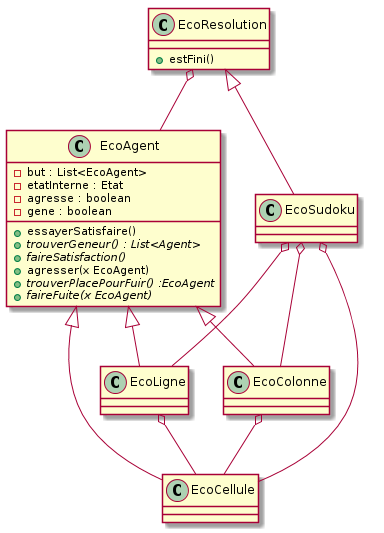
\includegraphics[scale=0.7]{diagrams/ecoResolution.png}
            \end{center} 

            Pour l'éco-résolution, nous retrouvons une seule méthode estFini(), qui vérifie lorsque tous les éco-agents de notre système sont satisfaits. \\
            Avant de démarrer l'éco-résolution, nous allons compléter les cases vides de notre sudoku. Les cases étant déjà dans l'énoncé comporteront un attribut cellType valant "GIVEN". Pour remplir notre sudoku, nous allons effectué un remplissage "intelligent", c'est-à-dire que dans chaque bloc nous allons placer une et une seule fois chaque numéro de 1 à 9.\\
            Nous avons choisi que nos cellules, nos lignes et nos colonnes seraient considérés comme éco-agent. \\
            \subsubsection{Les lignes}
                Nous allons voir les lignes comme éco-agent de la manière suivante : \\
                \begin{itemize}
                    \item Le but d'une ligne est que tous les éco-agents qui la compose (cellule) aient des numéros différents.
                    \item Pour trouver les gêneurs, cela correspondra à toutes les cellules qui ont un numéro qui intervient plus d'une fois. 
                    \item FaireSatisfaction : Passer l'état comme étant satisfait
                    \item une ligne ne pourra ni fuir, ni être en recherche de fuite.   
                \end{itemize}
            \subsubsection{Les colonnes}
                Nous allons voir les colonnes comme éco-agent de la manière suivante, analogue à la façon dont nous voyons les lignes : \\
                \begin{itemize}
                    \item Le but d'une colonne est que tous les éco-agents qui la compose (cellule) aient des numéros différents.
                    \item Pour trouver les gêneurs, cela correspondra à toutes les cellules qui ont un numéro qui intervient plus d'une fois. 
                    \item FaireSatisfaction : Passer l'état comme étant satisfait
                    \item une colonne ne pourra ni fuir, ni être en recherche de fuite.   
                \end{itemize}
            \subsubsection{Les cellules}
                Nous allons voir les cellules comme des agents de la manière suivante : 
                \begin{itemize}
                    \item Une cellule est satisfaite si sa ligne et sa colonne sont satisfaites
                    \item Les gêneurs d'une cellule sont les numéros ayant la même valeur sur la colonne et la ligne
                    \item Pour FaireSatisfaction d'une cellule, il faut qu'il n'y ai plus de gêneur
                    \item Pour trouverPlacePourFuir d'une cellule nous avons plusieurs idées : choisir une cellule aléatoirement dans le même bloc, choisir une cellule aléatoirement dans le bloc mais qui ne soit pas sur la ligne ou colonne de notre agent qui lance l'agression et enfin choisir la cellule qui a le plus de gêne.
                    \item Pour faireFuite, nous allons échanger les numéros de nos deux cellules.
                \end{itemize}
        \subsection{Diagramme de séquence}
            \subsubsection{SeSatisfaire}
                \begin{center}
                    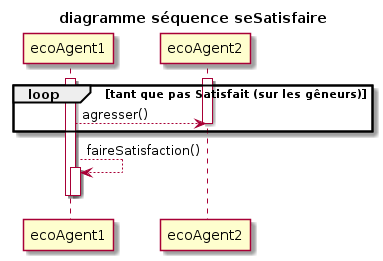
\includegraphics[scale=0.7]{diagrams/sequenceEcoResolution1.png}
                \end{center} 
                Pour se satisfaire un éco-agent agresse tous les autres agents qui le gênent. Une fois qu'il n'est plus gêné il est satisfait. 
            \subsubsection{Fuir}
                \begin{center}
                    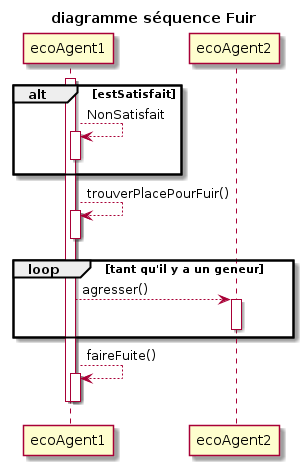
\includegraphics[scale=0.7]{diagrams/sequenceEcoResolution2.png}
                \end{center} 
                Si un agent doit fuir et qu'il est satisfait il devient non satisfait. Ensuite il recherche une place pour fuir, agresse tous les gêneurs qui l'empêche de fuir puis fait fuite. 
